The results obtained with the embedding + K-NN solution are very promising, as we can see in Figure~\ref{fig:tSNE-plot}.
\begin{figure}
    \centering
    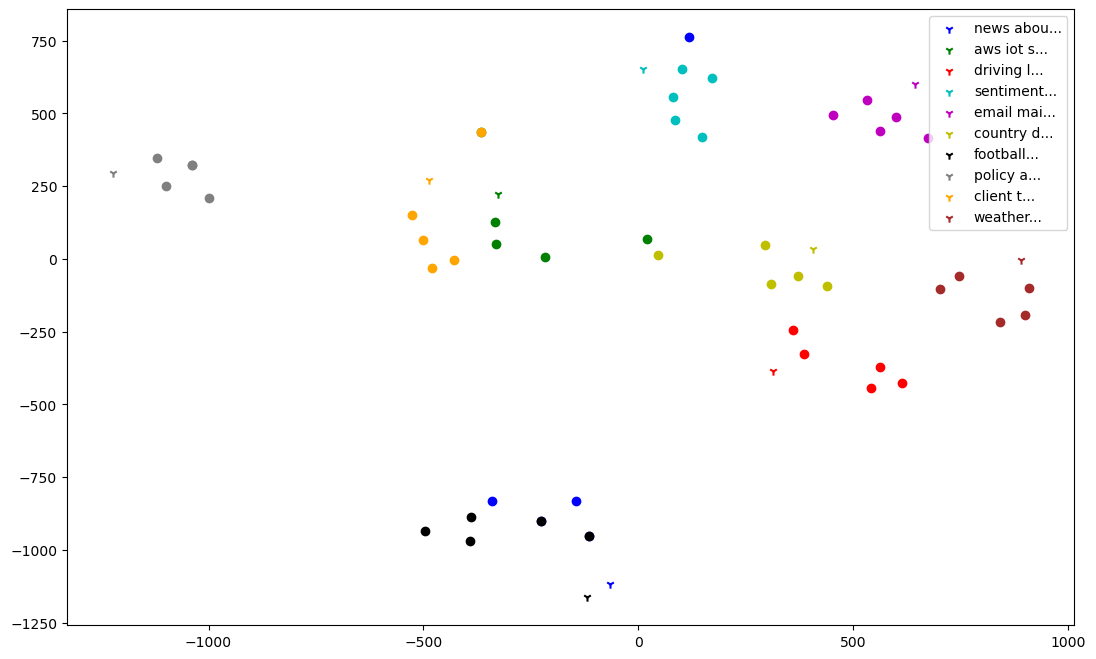
\includegraphics[width=13cm]{../out/plots/SNE}
    \caption{T-SNE Plot}
    \label{fig:tSNE-plot}
\end{figure}
With the \("\)Y\("\) markers representing the queries, and the dots representing the most similar documents found for that query, we can see that the dots and \("\)Y\("\) markers of the same colors are fairly close to each other. \\ \\
% TODO - Explain how the ground truth was computed
Moreover, we performed a validation step with a ground truth.
% TODO - Add reference to precision and recall definitions
From the validation step, we concluded that the average precision and recall of the document retrieval are:
\[P_a = 0.6 ~~~~~~ R = 1.0\]
This validation was done on 10 different queries.
The position in which each ground truth appeared in the searches can be found below.
\begin{verbatim}
  Position in which the ground truth was found:

      "NFL v3 Ply-by-Play" was found at position #1
      "AWS IoT Secure Tunneling" was found at position #4
      "Transport Department" was found at position #4
      "Text Analytics & Sentiment Analysis API | api.text2data.com" was
        found at position #4
      "MailboxValidator Free Email Checker" was found at position #1
      "Interzoid Country Data Standardization API" was found at position #1
      "Soccer v3 Projections" was found at position #1
      "PolicyClient" was found at position #1
      "NetworkManagementClient" was found at position #3
      "Interzoid Get Weather City API" was found at position #2
\end{verbatim}
As we can see, all ground truths we found in the top 5 results -- hence $p = 1.0$.
The validation on the ground truth, though, does not paint the full picture of the capabilities this solution offers.
For example, if we try searching using the query: \("\)american sports news\("\), the top 5 documents returned by the information retrieval system will be the following.
\begin{verbatim}
  These are the top 5 results of the query "american sports news":

      1. NFL v3 Play-by-Play     v.1.0   [67%]
      2. News Plugin             v.1     [66%]
      3. Soccer v3 Projections   v.1.0   [64%]
      4. MLB v3 Projections      v.1.0   [64%]
      5. NFL v3 Scores           v.1.0   [64%]
\end{verbatim}
% TODO - Add dicussion on "american sports news" not being present in the specification
As we can see in the results above, the engine is able to recognize that both the \textit{NFL} and the \textit{MLB} are professional American sport leagues.
The former being the National Football League, and the latter being the Major League Baseball.
Moreover, it is also able to understand that soccer is a sport and return it. \\ \\
As can be seen both in the average precision ($P_a = 0.6$), and the above example, there are still some noisy results that match part or none of the queries, but this is acceptable.
The reason is that this is not the only means of searching.
% TODO - Further filtering from the result of the knn operation
In tandem with the natural language query, there is also a DSL that can be used to filter the documents and obtain a more accurate result.